\section{Graphics Card Simulations}

\par
The probabilistic approach described in the previous section created a significant performance increase. 
However, there are several significant factors which limit the feasibility of using similar methods for the rest of the detector, including;
\begin{itemize}
    \item Optical propagation is required to be performed at least once
    \item Other regions of the detector contain significantly more complex geometry
\end{itemize}
For example, if a probabilistic map were to be applied to the entire TPC Liquid Xenon region, several weeks worth of a full cluster would be required in order to produce the equivalent statistics.
Although there are ways in which this could be reduced - such as Z-line symmetry - the initial overhead remains impractically high.

\par
Instead, a different approach can be considered, but this involves understanding what is and isn't required in the simulation.
Optical photon simulations are relatively simple in that regard as there are no daughter particles that need to be tracked.
They do however have some probability of being absorbed and re-emitted during propagation.
Besides this, the photons can be considered to travel in a straight line until they reach a boundary.
The simulation is therefore dominated by intersection calculations, or \textit{"has the photon reached the edge of this material yet?"}.

\par
CPUs have typically been designed to minimise task latency; ie the time required to complete any given task.
This differs from GPU design where by maximum throughput is required. 
This is achieved by having individual poorer thread performance but by having more threads available.
Therefore to utilise a GPU effectively, the tasks being performed should be as independent as possible and requiring few resources.

\par
Optical photon simulations fit in to this category as each photon is independent of another, and is at the 'end of the processing line', so are simulated to propagate until they are; absorbed, hit a PMT or leave the detector universe.
Additionally, the physics is relatively simple.

\par
Before attempting to improve the speed of simulation, it is important to understand why simulation speed is limited on CPUs. 
LZ particle propagation simulations are performed in BACCARAT, a software package built upon GEANT4, in which the geometry is defined (as shown in Figure XXX).
GEANT4 geometry is defined as XXX.
GEANT4 based simulations are relatively slow because XXX.

There have been many different attempts to transfer this part of the simulation on to GPUs, such as Chroma \cite{chroma_presentation_ref}.
But they are all based on CUDA... XXX.



\par
NVIDIA OptiX is a general purpose ray-tracing framework.
The propagation of a ray is defined by a set of CUDA programs that handle the various steps of a rays journey; generation, object intersection and closest hit.
These programs are combined with geometry traversal functionality into a ray tracing kernel. 
This structure is used by the traversal algorithm to search for the primitives that potentially intersect a given ray.



\subsection{LZ Geometry in Geant4}
\par
BACCARAT is built upon Geant4 (G4) in which the LZ detector geometry is defined.
The detector is comprised primarily of two parts, solids and structures.
Solids are Constructive Solid Geometry (CSG) which are made up of primitive shapes such as cubes, spheres, cylinders, etc...
There are combined together using boolean operations (addition, subtraction) to crease the solids.
These solids are connected to each other by logical and physical volumes.
These define the location and rotation of the solid relative to other solids/volumes and the world volume.
A logical volume contains all of the information associated with a given solid(s) except the position and the rotation.
A physics volumes is made up from logical volumes and adds position.

\par
Geometry Description Markup Language (GDML) is an XML-based language which allows for a detectors geometry and associated physical properties to be exported with it.
This allows for the geometry created in Geant4 to be passed into any XML compatible framework and be used.
GDML is a subset of XML which is designed to describe the geometry by describing a detector as a series of trees which correspond to the hierarchy of volumes \cite{GDML_USER_GUIDE_ref}.

\par
Unfortunately OptiX is not natively XML compatible, 
The LZ XML geometry is read in and converted into a tree structure.
For each solid, a binary tree is defined with the tree consisting of nodes and leaves.
Each node represents a boolean operation and each leave is a primitive.
A simple binary tree in both a balanced form and unbalanced is shown in Figure \ref{fig:UnionSolidBinaryTree}.
The tree structures shown in Figure \ref{fig:UnionSolidBinaryTree} could describe the CSG example in.
For realistic geometries where solids are combined together, these stack on each other to the point where there is a root tree.
The root tree is the highest level structure definition.
The binary trees for each solid are combined together into one root tree.
Any node can have a transform associated with it as well.
This is a 4x4 matrix.


\subsection{Geometry on GPU}
\par
The key difference between Geant4 simulations and a ray-tracing approach is that rather than using the CSG volume tree, boundaries volume hierarchy (BVH) are used exclusively.
Essentially what this means is that the primitives which made up the solids are defined in terms of boundaries.

\par
In order for a primitive to be used within the OptiX 6.0 framework, the volume must be defined in two parts; boundary and intersection.
The boundary is the limits of the shape, ie at what point does the ray need to be checked if it might intersect with the surface.
The intersection is the calculation which is performed to evaluate to determine if the ray intercepts with the boundary.
A key point (might put this sentence later) is that the intersection needs to account of cases where the ray comes from inside the primitive as well as from the outside in order to be used in a CSG tree.


\begin{figure}[!htpb]
\centering 
\begin{tikzpicture}[level distance=1.5cm,
  level 1/.style={sibling distance=3cm},
  level 2/.style={sibling distance=1.5cm}]
  \node {u}
    child {node {u}
      child {node {u}
        child {node {ps}}
        child {node {ps}}}
      child {node {ps}}}
    child {node {ps}};
\end{tikzpicture}
\begin{tikzpicture}[level distance=1.5cm,
  level 1/.style={sibling distance=3cm},
  level 2/.style={sibling distance=1.5cm}]
  \node {u}
    child {node {u}
      child {node {ps}}
      child {node {ps}}
    }
    child {node {u}
    child {node {ps}}
      child {node {ps}}
    };
\end{tikzpicture}
\caption{Binary tree representation of a simple solid comprised of the union (u) of 4 primitive solids (ps). \textbf{Left:} Unbalanced tree. \textbf{Right:} Balanced tree.}
\label{fig:UnionSolidBinaryTree}
\end{figure}

\subsection{Translation of LZ geometry}
\par
The LZ geometry is comprised of in-excess of 900,000 shapes, and although there is some duplication, this only reduces down to around 14,000 shapes.
Additionally, a large number of these shapes are complex additions which 
Reducing the scope to only include the TPC and Skin decreases this to 9,000 unique shapes which is 30-times greater than that of JUNO or DayaBay.
\par
This in performed in a way as described in \cite{CSG_Intersection_ref}.

\par
The LZ geometry contains many large volumes which


\begin{figure}[!htbp]
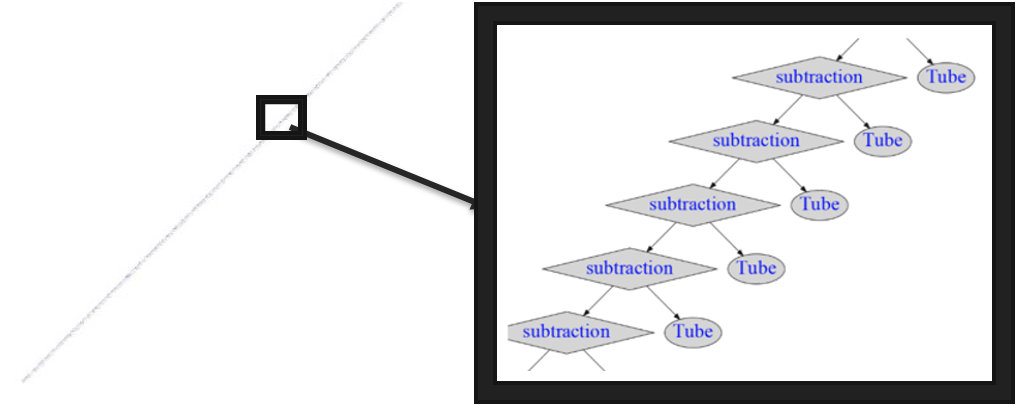
\includegraphics[width=\textwidth]{Figures/Simulations/unbalanced_ptfe.png}
\centering
\caption{Visual Representation of titanium top plate solid, comprised of a single G4Tube and 283 G4Tube subtractions. Kindly created by B. Krikler.}
\label{fig:Opticks_unbalanced_shape}
\end{figure}



\begin{figure}[!htbp]
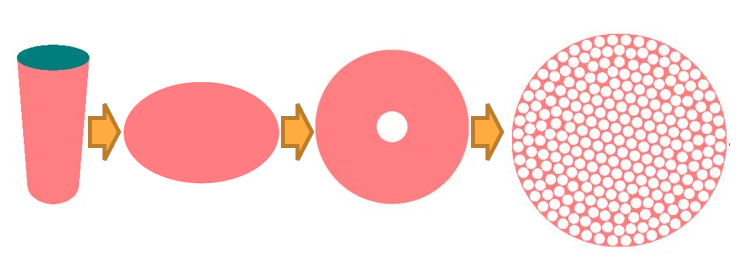
\includegraphics[width=0.7\textwidth]{Figures/Simulations/opticks_PTFE_primative.png}
\centering
\caption{Development stages for representing a 3D disc with multiple holes and a 2D disc with holes as defined within OptiX intersection program.}
\label{fig:Opticks_PTFE_primative}
\end{figure}


\begin{figure}[!htbp]
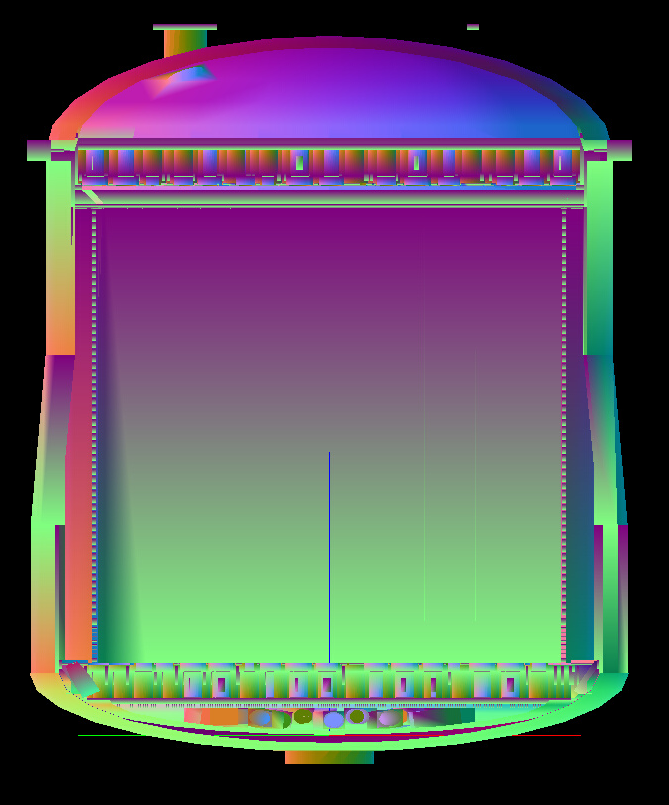
\includegraphics[width=8cm]{Figures/Simulations/LZ_In_Opticks.png}
\centering
\caption{TPC of LZ raytraced. Translated from Geant4 GDML file into NPY set using Opticks and viewed within Opticks via the OpenGL Buffer.
The blue, green and red lines towards the bottom of the figure are the axis.}
\label{fig:OpticksLZTPC}
\end{figure}

\par
To compare the optical photon propagation within the LZ geometry on Opticks with that from BACCARAT, a series of tests were devised.
As the initial purpose of this project was to simulate S2 photons, two S2 light maps were created using the same number of photons; XXXX million (15 billion I think).
Using a much of the same geometry as possible the simulations from BACCARAT and Opticks were compared.
This improvement 

\begin{figure}[!htbp]
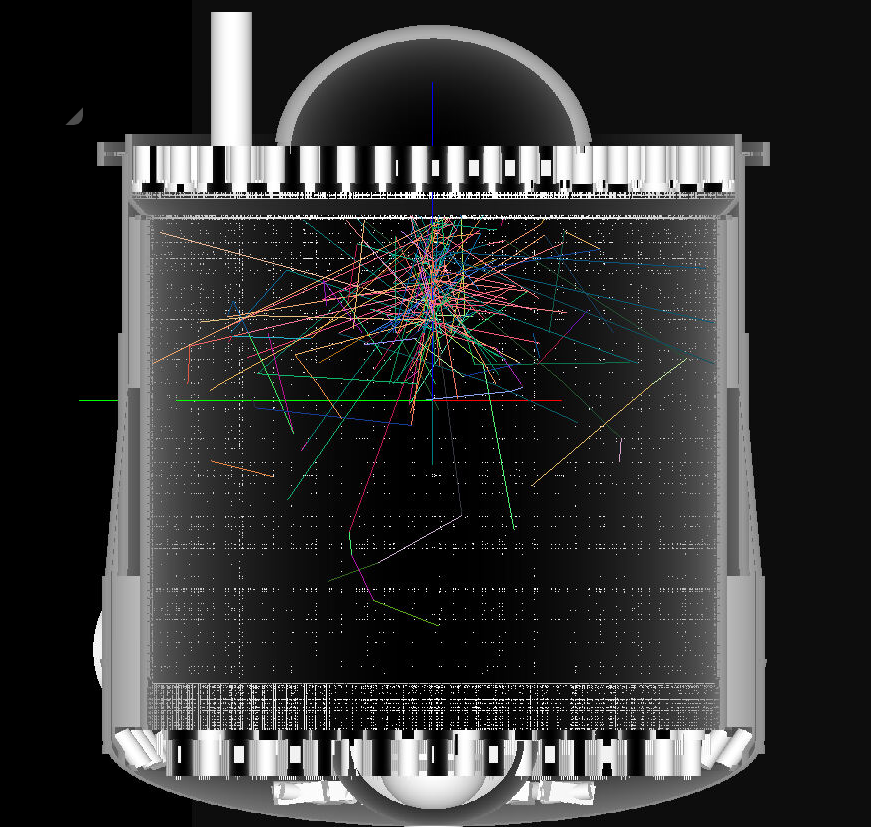
\includegraphics[width=10cm]{Figures/Simulations/LZ_S1_photons_In_Opticks.png}
\centering
\caption{TPC of LZ raytraced. Translated from Geant4 GDML file into NPY set using Opticks and viewed within Opticks via the OpenGL Buffer.
The blue, green and red lines extended outside the OCV are the axis. After each reflection a photons colour has been set to change.}
\label{fig:OpticksLZTPC_S1_Photons}
\end{figure}

\par
On a Tesla T4 GPU, after a 4-minute initialisation time using the serialised geometry, 200,000 photons per second were generated and propagated.
This marks a 720x improvement over single-core Geant4 propagation where 277 photons per second were generated and propagated for the S2 Light Map or 360x improvement over the expected gain when compared to GEANT4.
This improvement highlights one of the reasons for choosing an OptiX-based approach rather than pure CUDA, as the improvement would have been closer to 200x such as was shown in \cite{chroma_presentation_ref}.
However, it still lacks behind the improvement demonstrated using Opticks in \cite{Opticks_CHEP_2019_ref}, though this is primarily due to higher grade GPUs being used with RTX-cores.

\par
The LZ collaboration is continuing to develop upon this work with an integration plan into the simulation chain \cite{SEriksen_Opticks_CHEP_2021_ref, SEriksen_IoP_2021_talk_ref, lz_status_with_opticks_ref}.
Additionally, as this work was performed using NVIDIA OptiX 6.5.0, newer features available in 7.0.0+ will allow even greater performance and better use of compute-cluster GPU setup.
TODO CITE.
The primary limitation has been upon an improved GDML writer and reader in Geant4, requireing the LZ simulation package to update. 
However, with the planning for Gen-3 direct detection dark matter experiments, the optical photons will continue to be a limitation and are already being considered \cite{DARWIN_GPU_simulations_2022_ref,  accelerated_bvh_ref}.